\documentclass{article}
\usepackage{tikz}
\usetikzlibrary{shapes.geometric, arrows, positioning}
\begin{document}
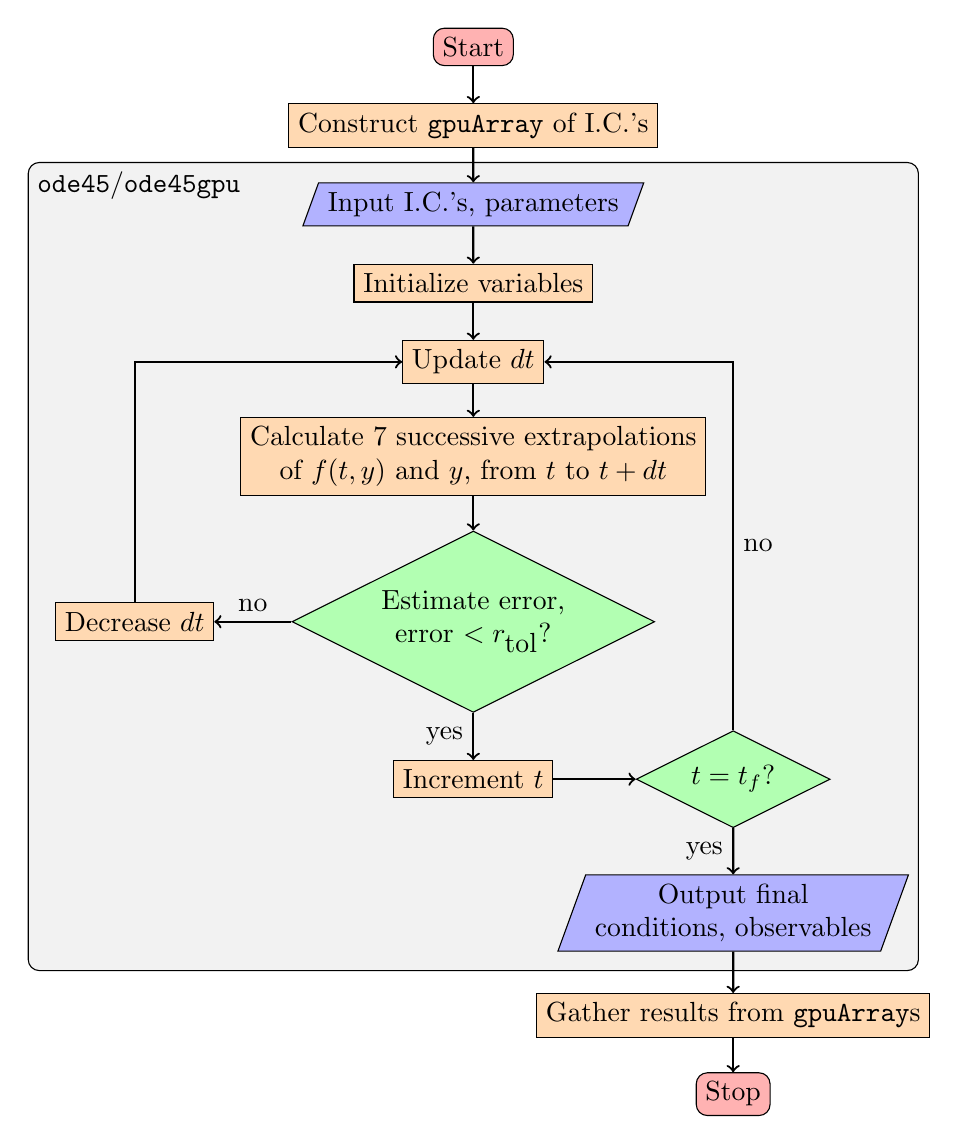
\begin{tikzpicture}
    \tikzstyle{startstop} = [rectangle, rounded corners, draw, fill=red!30]
    \tikzstyle{io} = [trapezium, trapezium left angle=70, trapezium right angle=110, draw, fill=blue!30]
    \tikzstyle{arrow} = [->,thick]
    \tikzstyle{process} = [rectangle, draw, fill=orange!30]
    \tikzstyle{decision} = [diamond, aspect=2, draw, fill=green!30]
    \tikzstyle{blockjusttext} = [rectangle, text width=31.5em, rounded corners]
    \tikzstyle{blockfill} = [rectangle, draw, fill=gray!10, text width=31.5em, rounded corners, minimum height=29.2em]
    \node (start) [startstop] {Start};
    \node (gpuArray) [process, below of=start] {Construct \verb+gpuArray+ of I.C.'s};
    \node (back) [blockfill, below=0.5em of gpuArray] {};
    \node (label) [blockjusttext, below=0.5em of gpuArray] {\verb+ode45+/\verb+ode45gpu+};
    \node (in) [io, below of=gpuArray] {Input I.C.'s, parameters};
    \node (init) [process, below of=in] {Initialize variables};
    \node (update) [process, below of=init] {Update $dt$};
    \node[align=center] (7) [process, below of=update, node distance=1.2cm] {Calculate 7 successive extrapolations\\of $f(t,y)$ and $y$, from $t$ to $t+dt$};
    \node[align=center] (dec) [decision, below of=7, node distance=2.1cm] {Estimate error,\\error $<r_\textrm{tol}$?};
    \node (decdt) [process, left of=dec, node distance=4.3cm] {Decrease $dt$};
    \node (inct) [process, below of=dec, node distance=2.0cm] {Increment $t$};
    \node (tf) [decision, right of=inct, node distance=3.3cm] {$t=t_f$?};
    \node[align=center] (final) [io, below of=tf, node distance=1.7cm] {Output final\\conditions, observables};
    \node (gather) [process, below of=final, node distance=1.3cm] {Gather results from \verb+gpuArray+s};
    \node (stop) [startstop, below of=gather] {Stop};
    \draw [arrow] (start) -- (gpuArray);
    \draw [arrow] (gpuArray) -- (in);
    \draw [arrow] (in) -- (init);
    \draw [arrow] (init) -- (update);
    \draw [arrow] (update) -- (7);
    \draw [arrow] (7) -- (dec);
    \draw [arrow] (dec) -- node[anchor=south] {no} (decdt);
    \draw [arrow] (decdt) |- (update);
    \draw [arrow] (dec) -- node[anchor=east] {yes} (inct);
    \draw [arrow] (inct) -- (tf);
    \draw [arrow] (tf) |- node[near start, anchor=west] {no} (update);
    \draw [arrow] (tf) -- node[anchor=east] {yes} (final);
    \draw [arrow] (final) -- (gather);
    \draw [arrow] (gather) -- (stop);
\end{tikzpicture}
\end{document}
